\documentclass[times, utf8, zavrsni]{fer}
\usepackage{booktabs}
\usepackage{tikz}
\usepackage{algorithmic}
\usepackage{algorithm}
\usepackage{listings}
\usepackage{amsthm}
\newtheorem{theorem}{Teorem}[section]

\begin{document}

\thesisnumber{253}

\title{Prebrojavanje razapinjućih stabala grafa}

\author{Dorian Kablar}

\maketitle

% Ispis stranice s napomenom o umetanju izvornika rada. Uklonite naredbu \izvornik ako želite izbaciti tu stranicu.

% Dodavanje zahvale ili prazne stranice. Ako ne želite dodati zahvalu, naredbu ostavite radi prazne stranice.
\zahvala{Zahvaljujem mentorici, doc. dr. sc. Anamari Nakić, na motivaciji i savjetima prilikom pisanja ovog rada.

Zahvaljuem svojim roditeljima, pogotovo majci, koji su me podržavali u svakoj odluci, i koji su uvijek znali kako pomoći, čak i kad nisam bio svjestan da je pomoć potrebna.}

\tableofcontents

\chapter{Uvod}
U prvom dijelu ću iznijeti glavne definicije i rezultate vezane uz grafove i stabla. U drugom dijelu će biti govora o razapinjućim stablima. Pritom ću iznijeti neke osnovne rezultate te primjere teorijskog računanja broja razapinjučih stabala. 
U trećem dijelu ću iskazati i dokazati matrični teorem o stablima. 

U četvrtom dijelu ću, koristeći prethodno dokazani teorem, iznijeti rezultate za primjere pojedinačnih grafova, kao i za grafove s proizvoljnim brojem vrhova, n. U petom dijelu, bit će opisan relevantan (za razapinjuća stabla) dio aplikacije \textit{Graphelite} koja je razvijena u sklopu kolegija \textit{Projekt R} u 5. semestru, te će se na primjerima prikazati njezin rad. Naposljetku će biti donesen zaključak o svemu što je napravljeno.

\chapter{Glavne definicije i rezultati}

\chapter{Razapinjuća stabla}

\section{Broj razapinjućih stabala - primjeri}

U ovom odjeljku bavit ću se određivanjem eksplicitnih formula za računanje broja razapinjućih stabala određenih vrsta grafova. Karakteristika tih formula će biti ta da će jedina varijabla u njima biti \textit{n}, odnosno broj vrhova grafa.

\subsection{Kotač, \textit{W\textsubscript{n}}}

Prvi primjer je graf kotač, odnosno \textit{W\textsubscript{n}}. Kotač je graf koji je sličan grafu ciklusu \textit{C\textsubscript{n}} uz razliku da se jedan od vrhova nalazi u sredini te su svi ostali vrhovi, osim što su povezani u ciklus, još povezani s vrhom u sredini.

\begin{figure}[htb]
	\centering
	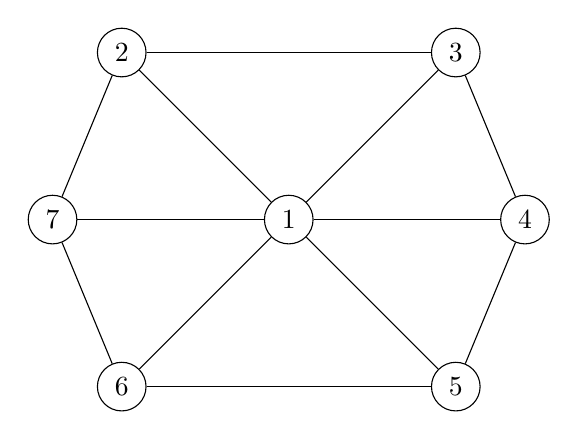
\begin{tikzpicture}[node distance={30mm}, main/.style = {draw, circle}] 
		\node[main] (1) {$1$}; 
		\node[main] (2) [above left of=1] {$2$};
		\node[main] (3) [above right of=1] {$3$};
		\node[main] (4) [right of=1] {$4$};
		\node[main] (5) [below right of=1] {$5$};
		\node[main] (6) [below left of=1] {$6$};
		\node[main] (7) [left of=1] {$7$};
		\draw (1) -- (2);
		\draw (1) -- (3);
		\draw (1) -- (4);
		\draw (1) -- (5);
		\draw (1) -- (6);
		\draw (1) -- (7);
		\draw (2) -- (3);
		\draw (3) -- (4);
		\draw (4) -- (5);
		\draw (5) -- (6);
		\draw (6) -- (7);
		\draw (7) -- (2);
	\end{tikzpicture}
	\caption{Kotač $W_6$}
\end{figure}

Jedan primjer kotača je i $W_6$ prikazan na slici 3.1.

Za računanje će od iznimne važnosti biti sljedeći izraz:

\begin{equation}
	T(G) = T(G - e) + T(G \backslash e)
\end{equation}

Prije samog izračuna, potrebno je dokazati da je izraz (3.1) ispravan.

\begin{proof}
Neka je \textit{e} neki fiksni brid od \textit{G}. Uočimo da se razapinjuća stabla od \textit{G} dijele na:
\begin{itemize}
	\item razapinjuća stabla od \textit{G} koja ne sadrže brid \textit{e}; neka je taj broj jednak x,
	\item razapinjuća stabla od \textit{G} koja sadrže brid \textit{e}; neka je taj broj jednak y.
\end{itemize}
Vrijedi: $T(G) = x + y$. Uočimo sada da je:
\begin{itemize}
	\item $x = T(G - e)$ jer je svako razapinjuće stablo od \textit{G} koje ne sadrži \textit{e}, ujedno i razapinjuće stablo od $G - e$
	\item $y = T(G \backslash e)$ jer svako razapinjuće stablo od $G \backslash e$ možemo dobiti iz razapinjućeg stabla od \textit{G} koje sadrži brid \textit{e} postupkom konkatenacije brida \textit{e} u tom stablu.
\end{itemize}
Dakle, vrijedi $T(G) = T(G - e) + T(G \backslash e)$.
\end{proof}

Da bismo mogli pronaći eksplicitnu formulu za računanje broja razapinjućih stabala kotača s proizvoljnim brojem vrhova, potrebno je definirati nekoliko familija grafova koje ćemo koristiti.

\begin{figure}[htb]
	\minipage{0.33\textwidth}
	\begin{center}
		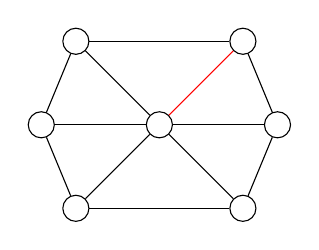
\begin{tikzpicture}[node distance={15mm}, main/.style = {draw, circle}] 
			\node[main] (1) {}; 
			\node[main] (2) [above left of=1] {};
			\node[main] (3) [above right of=1] {};
			\node[main] (4) [right of=1] {};
			\node[main] (5) [below right of=1] {};
			\node[main] (6) [below left of=1] {};
			\node[main] (7) [left of=1] {};
			\draw (1) -- (2);
			\draw[red] (1) -- (3);
			\draw (1) -- (4);
			\draw (1) -- (5);
			\draw (1) -- (6);
			\draw (1) -- (7);
			\draw (2) -- (3);
			\draw (3) -- (4);
			\draw (4) -- (5);
			\draw (5) -- (6);
			\draw (6) -- (7);
			\draw (7) -- (2);
		\end{tikzpicture}
	\end{center}
	\caption*{\textit{$W_n$}}
	\endminipage\hfill
	\minipage{0.33\textwidth}
	\begin{center}
		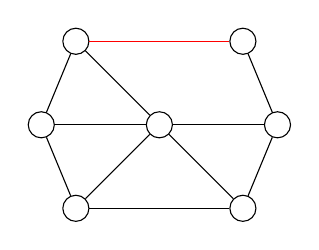
\begin{tikzpicture}[node distance={15mm}, main/.style = {draw, 	circle}] 
			\node[main] (1) {}; 
			\node[main] (2) [above left of=1] {};
			\node[main] (3) [above right of=1] {};
			\node[main] (4) [right of=1] {};
			\node[main] (5) [below right of=1] {};
			\node[main] (6) [below left of=1] {};
			\node[main] (7) [left of=1] {};
			\draw (1) -- (2);
			\draw (1) -- (4);
			\draw (1) -- (5);
			\draw (1) -- (6);
			\draw (1) -- (7);
			\draw[red] (2) -- (3);
			\draw (3) -- (4);
			\draw (4) -- (5);
			\draw (5) -- (6);
			\draw (6) -- (7);
			\draw (7) -- (2);
		\end{tikzpicture}
	\end{center}
	\caption*{$A_n$}
	\endminipage\hfill
	\minipage{0.33\textwidth}
	\begin{center}
		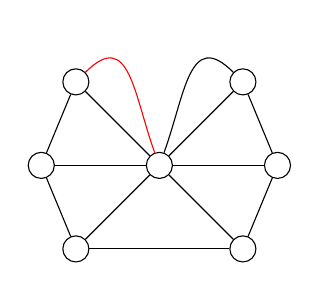
\begin{tikzpicture}[node distance={15mm}, main/.style = {draw, 	circle}] 
			\node[main] (1) {}; 
			\node[main] (2) [above left of=1] {};
			\node[main] (3) [above right of=1] {};
			\node[main] (4) [right of=1] {};
			\node[main] (5) [below right of=1] {};
			\node[main] (6) [below left of=1] {};
			\node[main] (7) [left of=1] {};
			\draw (1) -- (2);
			\draw (1) -- (3);
			\draw (1) -- (4);
			\draw[red] (1) to [out=110,in=45,looseness=1.5] (2);
			\draw (1) to [out=70,in=135,looseness=1.5] (3);
			\draw (1) -- (5);
			\draw (1) -- (6);
			\draw (1) -- (7);
			\draw (3) -- (4);
			\draw (4) -- (5);
			\draw (5) -- (6);
			\draw (6) -- (7);
			\draw (7) -- (2);
		\end{tikzpicture}
	\end{center}
	\caption*{$B_n$}
	\endminipage\hfill
	\minipage{0.5\textwidth}
	\begin{center}
		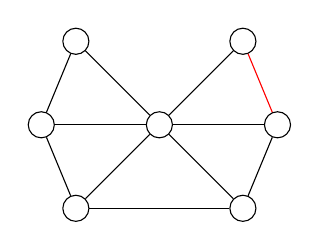
\begin{tikzpicture}[node distance={15mm}, main/.style = {draw, 	circle}] 
			\node[main] (1) {}; 
			\node[main] (2) [above left of=1] {};
			\node[main] (3) [above right of=1] {};
			\node[main] (4) [right of=1] {};
			\node[main] (5) [below right of=1] {};
			\node[main] (6) [below left of=1] {};
			\node[main] (7) [left of=1] {};
			\draw (1) -- (2);
			\draw (1) -- (3);
			\draw (1) -- (4);
			\draw (1) -- (5);
			\draw (1) -- (6);
			\draw (1) -- (7);
			\draw[red] (3) -- (4);
			\draw (4) -- (5);
			\draw (5) -- (6);
			\draw (6) -- (7);
			\draw (7) -- (2);
		\end{tikzpicture}
	\end{center}
	\caption*{$C_n$}
	\endminipage\hfill
	\minipage{0.5\textwidth}
	\begin{center}
		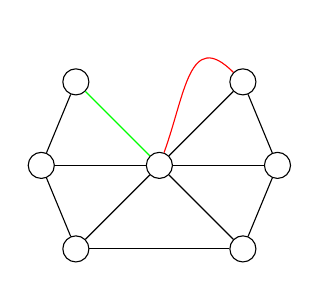
\begin{tikzpicture}[node distance={15mm}, main/.style = {draw, 	circle}] 
			\node[main] (1) {}; 
			\node[main] (2) [above left of=1] {};
			\node[main] (3) [above right of=1] {};
			\node[main] (4) [right of=1] {};
			\node[main] (5) [below right of=1] {};
			\node[main] (6) [below left of=1] {};
			\node[main] (7) [left of=1] {};
			\draw[green] (1) -- (2);
			\draw (1) -- (3);
			\draw (1) -- (4);
			\draw[red] (1) to [out=70,in=135,looseness=1.5] (3);
			\draw (1) -- (5);
			\draw (1) -- (6);
			\draw (1) -- (7);
			\draw (3) -- (4);
			\draw (4) -- (5);
			\draw (5) -- (6);
			\draw (6) -- (7);
			\draw (7) -- (2);
		\end{tikzpicture}
	\end{center}
	\caption*{$D_n$}
	\endminipage\hfill
	\caption{Pet familija grafova koje će se koristiti za nalaženje eksplicitne formule za računanje broja razapinjućih stabala grafa kotača $W_n$ ($n$ označava broj vrhova).}
\end{figure}

Koristimo izraz (3.1) nad označenim bridovima sa slike 3.2, te dobivamo sustav rekurzivnih relacija:

$T(W_n) = T(A_n) + T(B_{n - 1})$

$T(A_n) = T(C_{n - 1}) + T(W_{n - 1})$

$T(B_n) = T(D_n) + T(B_{n - 1})$

$T(C_n) = T(C_{n - 1}) + T(D_{n - 1})$

$T(D_n) = T(C_n) + T(D_{n - 1}) = T(D_{n - 1}) + T(B_{n - 1})$

Uzmimo sada u obzir relacije za $T(C_n)$ i $T(D_n)$. Dobivamo:

\[T(C_{n + 1}) = T(C_n) + T(D_n) = 2T(C_n) + T(D_{n - 1}) = 3T(C_n) - T(C_{n - 1})\]
ili 
\[T(C_{n + 1}) - 3T(C_n) + T(C_{n - 1}) = 0\]
odnosno
\[T(C_n) - 3T(C_{n - 1}) + T(C_{n - 2}) = 0\] i
\[T(C_{n-1}) - 3T(C_{n - 2}) + T(C_{n - 3}) = 0\]

Oduzmemo li prethodne dvije relacije, dobit ćemo konačnu rekurzivnu relaciju za $T(C_n)$:

\[T(C_n) - 4T(C_{n - 1}) + 4T(C_{n - 2}) - T(C_{n - 3}) = 0\]

Promotrimo sada relacije za $T(W_n)$ i $T(A_n)$. Obzirom da je $T(B_{n -1}) = T(C_n)$, imamo $T(W_n) = T(A_n) + T(C_n)$ i, posljedično, $T(W_{n - 1}) = T(A_{n - 1}) + T(C_{n - 1})$.

Supstitucijom u relaciju $T(A_n) = T(C_{n - 1}) + T(W_{n - 1})$ dobivamo:

\[T(A_n) = T(A_{n - 1}) + 2T(C_{n - 1})\]
\[T(A_n) - T(A_{n - 1}) = 2T(C_{n - 1})\]

Obzirom da je $T(C_{n - 1}) - 3T(C_{n - 2}) + T(C_{n - 3}) = 0$, imamo:

\[2T(C_{n - 1}) - 2(3)T(C_{n - 2}) + 2T(C_{n - 3}) = 0\]
\[[T(A_n) - T(A_{n - 1})] - 3[T(A_{n - 1}) - T(A_{n - 2})] + [T(A_{n - 2}) - T(A_{n - 3})] = 0\]

iz čega, sređivanjem izraza, slijedi:

\[T(A_n) - 4T(A_{n - 1}) + 4T(A_{n - 2}) - T(A_{n - 3}) = 0\]

što je konačna rekurzivna relacija za $T(A_n)$.

Primjetimo da sada i $T(A_n)$ i $T(C_n)$ imaju homogenu rekurzivnu relaciju trećeg reda:

\[x_n - 4x_{n - 1} + 4x_{n - 2} - x_{n - 3} = 0\]

iz čega proizlazi da i $T(W_n) = T(A_n) + T(C_n)$ mora imati identičnu relaciju. Karakteristična jednadžba koja korespondira s ovom relacijom je:

\[r^3 - 4r^2 + 4r + 1 = 0\]
\[(r - 1)(r^2 - 3r + 1) = 0\]

Ta jednadžba ima karakteristične korijene $r_1 = \dfrac{3 + \sqrt{5}}{2}$, $r_2 = \dfrac{3 - \sqrt{5}}{2}$ i $r_3 = 1$. Dakle, opće rješenje od $T(W_n)$ je:

\[T(W_n) = \alpha(\dfrac{3 + \sqrt{5}}{2})^n + \beta(\dfrac{3 - \sqrt{5}}{2})^n + \gamma\]

Da bi se ova relacija rješila, potrebno je pronaći vrijednosti konstanti $\alpha$, $\beta$ i $\gamma$ takvih da se opće rješenje slaže s početnim uvjetima $T(W_3) = 16$, $T(W_4) = 45$ i $T(W_5) = 121$ (uz uvjet $n >= 3$). Dobivamo sustav:

\[T(W_n) = \alpha(\dfrac{3 + \sqrt{5}}{2})^3 + \beta(\dfrac{3 - \sqrt{5}}{2})^3 + \gamma = 16\]
\[T(W_n) = \alpha(\dfrac{3 + \sqrt{5}}{2})^4 + \beta(\dfrac{3 - \sqrt{5}}{2})^4 + \gamma = 45\]
\[T(W_n) = \alpha(\dfrac{3 + \sqrt{5}}{2})^5 + \beta(\dfrac{3 - \sqrt{5}}{2})^5 + \gamma = 121\]

Sustav se može rješiti na razne načine, jedan od njih je i preko matrice sustava:

\[
\centering 
\begin{bmatrix}
	\begin{array}{ccc|c}
		(\dfrac{3 + \sqrt{5}}{2})^3 & (\dfrac{3 - \sqrt{5}}{2})^3 & 1 & 16 \\
		(\dfrac{3 + \sqrt{5}}{2})^4 & (\dfrac{3 - \sqrt{5}}{2})^4 & 1 & 45 \\
		(\dfrac{3 + \sqrt{5}}{2})^5 & (\dfrac{3 - \sqrt{5}}{2})^5 & 1 & 121 \\
	\end{array}
\end{bmatrix}
\]

Cilj je da na lijevoj strani ostane jedinična matrica, i onda će vrijednosti s desne strane biti rješenja sustava. Ovaj sustav ima jedinstveno rješenje $\alpha = \beta = 1$ i $\gamma = -2$ iz čega slijedi da je broj razapinjučih stabala grafa kotača $W_n$ jednak:

\begin{equation}
T(W_n) = (\dfrac{3 + \sqrt{5}}{2})^n + (\dfrac{3 - \sqrt{5}}{2})^n - 2
\end{equation}

\chapter{Matrični teorem o stablima}

Cilj ovog poglavlja je izvesti rezultat koji broj razapinjućih stabala grafa računa kao determinantu matrice čije vrijednosti ovise o grafu. Te matrice nazivaju se \textit{Laplacijani}.

\section{Laplacian}

Neka je G neusmjereni graf s \textit{n} vrhova, i neka \textit{d\textsubscript{i}} označuje stupanj vrha \textit{i}. \textit{Laplacian L} je modificirana verzija matrice susjedstva grafa G, definirana na sljedeći način:

$L_{ij} = d_i$ ako je \textit{i} = \textit{j}, $L_{ij} = -1$ ako su vrhovi \textit{i} i \textit{j} povezani, te $L_{ij} = 0$ inače.

\begin{figure}[htb]
	\centering
	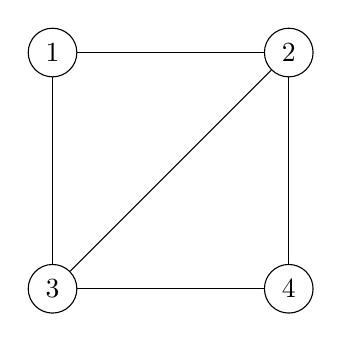
\begin{tikzpicture}[node distance={30mm}, main/.style = {draw, circle}] 
		\node[main] (1) {$1$}; 
		\node[main] (2) [right of=1] {$2$};
		\node[main] (3) [below of=1] {$3$};
		\node[main] (4) [below of=2] {$4$};
		\draw (1) -- (2);
		\draw (1) -- (3);
		\draw (2) -- (3);
		\draw (2) -- (4);
		\draw (3) -- (4);
	\end{tikzpicture}
	\caption{Primjer grafa s 4 vrha}
\end{figure}

Laplacian \textit{L} grafa sa slike 4.1 je:

\[
\centering
L = 
\begin{bmatrix}
	2 & -1 & -1 & 0 \\
	-1 & 3 & -1 & -1 \\
	-1 & -1 & 3 & -1 \\
	0 & -1 & -1 & 2
\end{bmatrix}
\]

Primjetimo da je suma svakog retka i stupca od \textit{L} jednak 0. Zbog toga je determinanta od \textit{L} uvijek jednaka 0.

Da bismo bili u mogućnosti iskazati matrični teorem o stablima, potrebno je uvesti još jedan komad notacije. Pretpostavimo li matricu \textit{A} s dimenzijama \textit{n} x \textit{n}, s \textit{A\textsuperscript{(ij)}} će se označavati matrica dimenzija (\textit{n} - 1) x (\textit{n} - 1) dobivena brisanjem \textit{i}-tog redka i \textit{j}-tog stupca matrice \textit{A}. Takve matrice se nazivaju \textit{minore}. Sljedeći teorem nam govori da nam minore \textit{Laplaciana} daju upravo rezultat koji tražimo.

\section{Matrix-Tree teorem}

\begin{theorem}[Matrix-Tree teorem]
Neka je G nepovezani graf ili multigraf i neka T(G) označava broj razapinjućih stabala u G. Za bilo koji i, T(G) = det L\textsuperscript{(ii)}, gdje je L laplacian od G. Preciznije, det L\textsuperscript{(ii)} je jednak za svaki i.
\end{theorem}

\begin{proof}
Teorem se dokazuje matematičkom indukcijom. Pretpostavimo da teorem vrijedi za povezane grafove s manje vrhova ili bridova. Kao bazu indukcije, pretpostavimo da se graf \textit{G} sastoji od samo jednog vrha. U tom slučaju, $T(G) = 1$, i teorem daje ispravan rezultat: $L = (0)$ i $L^{(11)}$ je matrica dimenzija 0 x 0, čija je determinanta po definiciji jednaka 1.

Za korak indukcije pretpostavljamo graf \textit{G} koji ima barem dva vrha, te odabiremo jedan od tih vrhova, recimo vrh \textit{i}. Ako \textit{i} nije incidentan s nijednim bridom, onda \textit{G} nema razapinjuće stablo. U ovom slučaju će teorem vrijediti jer je \textit{L\textsuperscript{(ii)}} zapravo \textit{Laplacian} ostatka grafa te će njezina determinanta biti jednaka nuli, kao što je navedeno u odjeljku 4.1.

\begin{figure}[htb]
	\minipage{0.33\textwidth}
	\begin{center}
		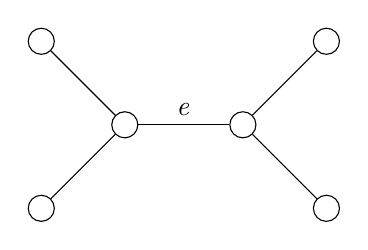
\begin{tikzpicture}[node distance={15mm}, main/.style = {draw, circle}] 
			\node[main] (1) {}; 
			\node[main] (2) [below right of=1] {};
			\node[main] (3) [right of=2] {};
			\node[main] (4) [above right of=3] {};
			\node[main] (5) [below left of=2] {};
			\node[main] (6) [below right of=3] {};
			\draw (1) -- (2);
			\draw (2) -- node[midway, above] {\textit{e}} (3);
			\draw (2) -- (5);
			\draw (3) -- (4);
			\draw (3) -- (6);
		\end{tikzpicture}
	\end{center}
	\caption*{\textit{G}}
	\endminipage\hfill
	\minipage{0.33\textwidth}
	\begin{center}
		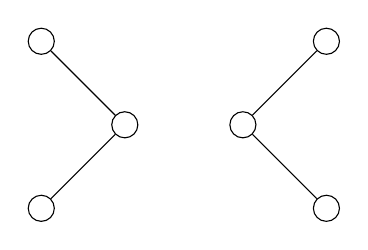
\begin{tikzpicture}[node distance={15mm}, main/.style = {draw, 	circle}] 
			\node[main] (1) {}; 
			\node[main] (2) [below right of=1] {};
			\node[main] (3) [right of=2] {};
			\node[main] (4) [above right of=3] {};
			\node[main] (5) [below left of=2] {};
			\node[main] (6) [below right of=3] {};
			\draw (1) -- (2);
			\draw (2) -- (5);
			\draw (3) -- (4);
			\draw (3) -- (6);
		\end{tikzpicture}
	\end{center}
	\caption*{\textit{G - e}}
	\endminipage\hfill
	\minipage{0.33\textwidth}
	\begin{center}
		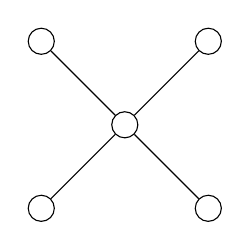
\begin{tikzpicture}[node distance={15mm}, main/.style = {draw, 	circle}] 
			\node[main] (1) {}; 
			\node[main] (2) [below right of=1] {};
			\node[main] (4) [above right of=2] {};
			\node[main] (5) [below left of=2] {};
			\node[main] (6) [below right of=2] {};
			\draw (1) -- (2);
			\draw (2) -- (5);
			\draw (2) -- (4);
			\draw (2) -- (6);
		\end{tikzpicture}
	\end{center}
	\caption*{$G \backslash e$}
	\endminipage\hfill
	\caption{$G - e$ je graf koji se dobije brisanjem brida \textit{e}, a $G \backslash e$ je graf koji se dobije kontrakcijom brida \textit{e} i spajanjem incidentnih vrhova u jedan vrh.}
\end{figure}

Sada pretpostavimo da je \textit{i} povezan s nekim drugim vrhom \textit{j}, te neka \textit{e} označava brid \textit{(i,j)}. Kao što je prikazano na slici 4.2, postoje dva načina na koje se može modificirati \textit{G}: brid \textit{e} možemo jednostavno izbrisati, ili možemo kontrakcijom vrhove \textit{i} i \textit{j} spojiti u jedan vrh. Takve grafove označujemo s $G - e$ i $G \backslash e$. Sada tvrdimo da je broj razapinjučih stabala \textit{T(G)} zadan sa sljedećim rekurzivnim izrazom:

\begin{equation}
	T(G) = T(G - e) + T(G \backslash e)
\end{equation}

Ispravnost izraza (4.1) je dokazana u poglavlju 3.

Prtpostavimo sada da matrični teorem vrijedi za $G - e$ i za $G \backslash e$. Možemo razmjestiti vrhove od \textit{G} tako da su \textit{i} i \textit{j} prva dva vrha. Sada Laplacian \textit{L} od \textit{G} možemo napisati kao:

\[
L_G =
\begin{bmatrix}
	\begin{array}{c|c|c}
		d_i & -1 & r_i^T \\
		\hline
		-1 & d_j & r_j^T \\
		\hline
		r_i & r_j & L'
	\end{array}
\end{bmatrix}
\]

Ovdje \textit{r\textsubscript{i}} i \textit{r\textsubscript{j}} predstavljaju \textit{(n - 2)}-dimenzionalne vektore koji opisuju konekcije vrhova \textit{i} i \textit{j} s ostalih \textit{n - 2} vrha od \textit{G} ($r_i^T$ i $r_j^T$ su transponirani vektori), a \textit{L'} je \textit{(n - 2)}-dimenzionalna minora koja predstavlja \textit{laplacian} ostatka grafa. \textit{Laplaciane} grafova $G - e$ i $G \backslash e$ pišemo na sljedeći način:

\[
L_{G - e} = 
\begin{bmatrix}
	\begin{array}{c|c|c}
		d_i - 1 & 0 & r_i^T \\
		\hline
		0 & d_j - 1 & r_j^T \\
		\hline
		r_i & r_j & L'
	\end{array}
\end{bmatrix},
L_{G \backslash e} = 
\begin{bmatrix}
	\begin{array}{c|c}
		d_i + d_j - 2 & r_i^T + r_j^T \\
		\hline
		r_i + r_j & L'
	\end{array}
\end{bmatrix}
\]

Da bi se indukcija završila, potrebno je pokazati:

\begin{equation}
	detL_G^{(ii)} = detL_{G - e}^{(ii)} + detL_{G \backslash e}^{(jj)}
\end{equation}

ili, u matričnom zapisu:

\[
det
\begin{pmatrix}
	\begin{array}{c|c}
		d_j & r_j^T \\
		\hline
		r_j & L'
	\end{array}
\end{pmatrix}
= det
\begin{pmatrix}
	\begin{array}{c|c}
		d_j - 1 & r_j^T \\
		\hline
		r_j & L'
	\end{array}
\end{pmatrix}
+ detL'.
\]

Ovaj rezultat slijedi iz činjenice da determinanta matrice može biti napisana kao linearna kombinacija njenih \textit{kofaktora}, tj. determinanti njenih minora. Za bilo koju matricu \textit{A} vrijedi

\begin{equation}
	detA = \sum_{j = 1}^{n} (-1)^j A_{1,j} detA^{(1,j)}.
\end{equation}

Dakle, ako se dvije matrice razlikuju samo u njihovim (1,1) ćelijama, a $A_{ij} = B_{ij}$ za svaki drugi \textit{i} i \textit{j}, njihove determinante se razlikuju za determinantu njigovih (1,1) minora, odnosno $detA = detB + detA^{(1,1)}.$ Primjenimo li ovo za $L_G^{(ii)}$ i $L_{G - e}^{(ii)}$, dobit ćemo izraz (4.2), čime se dovršava dokaz ovog teorema.
\end{proof}

\chapter{Računanje broja razapinjućih stabala pomoću matričnog teorema o stablima}

Da bismo se uvjerili da je rezultat prethodnog teorema zaista ispravan, u ovom poglavlju razraditi ćemo primjere.

\begin{figure}[htb]
	\centering
	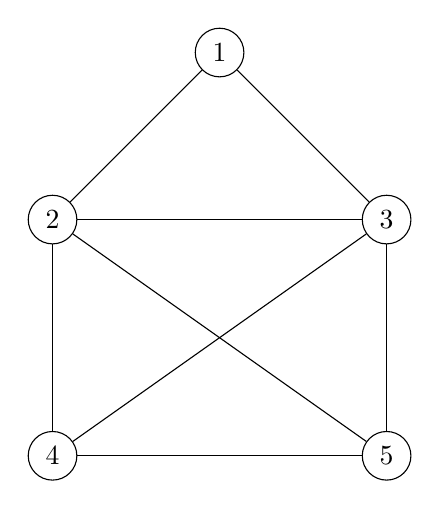
\begin{tikzpicture}[node distance={30mm}, main/.style = {draw, circle}] 
		\node[main] (1) {$1$}; 
		\node[main] (2) [below left of=1] {$2$};
		\node[main] (3) [below right of=1] {$3$};
		\node[main] (4) [below of=2] {$4$};
		\node[main] (5) [below of=3] {$5$};
		\draw (1) -- (2);
		\draw (1) -- (3);
		\draw (2) -- (3);
		\draw (2) -- (4);
		\draw (2) -- (5);
		\draw (3) -- (4);
		\draw (3) -- (5);
		\draw (4) -- (5);
	\end{tikzpicture}
	\caption{Primjer grafa s 5 vrhova}
\end{figure}

Na slici 5.1 prikazan je graf s 5 vrhova. Matrica susjedstva \textit{A} navedenog grafa, te njezin laplacian \textit{L} su sljedeći:

\[
\centering
A = 
\begin{bmatrix}
	0 & 1 & 1 & 0 & 0 \\
	1 & 0 & 1 & 1 & 1 \\
	1 & 1 & 0 & 1 & 1 \\
	0 & 1 & 1 & 0 & 1 \\
	0 & 1 & 1 & 1 & 0
\end{bmatrix}
,
L = 
\begin{bmatrix}
	2 & -1 & -1 & 0 & 0 \\
	-1 & 4 & -1 & -1 & -1 \\
	-1 & -1 & 4 & -1 & -1 \\
	0 & -1 & -1 & 3 & -1 \\
	0 & -1 & -1 & -1 & 3
\end{bmatrix}
\]

Kao sljedeći korak, stvorimo, na primjer, matricu \textit{L\textsuperscript{(22)}} dobivenu brisanjem drugog retka i drugog stupca matrice \textit{L}.

\[
\centering
L^{(22)} = 
\begin{bmatrix}
	2 & -1 & 0 & 0 \\
	-1 & 4 & -1 & -1 \\
	0 & -1 & 3 & -1 \\
	0 & -1 & -1 & 3
\end{bmatrix}
\]

Determinanta prethodne matrice, a ujedno i broj razapinjućih stabala grafa sa slike 5.1 je: $T(G) = det L^{(22)} = 40$. Jednak bi se rezultat dobio da smo matricu \textit{L\textsuperscript{(ii)}} stvorili tako da smo maknuli bilo koji drugi redak i stupac matrice \textit{L}.

\chapter{Graphelite - računanje broja razapinjućih stabala}

\textit{\textbf{Graphelite}} je web-aplikacija razvijena u 5. semestru u sklopu kolegija \textit{Projekt R} u suradnji s još dvoje kolega. To je aplikacija koja korisniku dopušta da crta jednostavne grafove i nad njima provodi razne algoritme i dobije zanimljive rezultate o nacrtanim grafovima. Moguće je crtati grafove, nacrtanom grafu odrediti najmanje razapinjuće stablo, odrediti duljinu struka (najkraći ciklus), odrediti kromatski broj, obojati vrhove grafa, te izračunati broj razapinjućih stabala.

\section{Računanje broja razapinjućih stabala grafa}

Broj razapinjućih stabala grafa kojeg korisnik nacrta u aplikaciji se računa pomoću matričnog teorema o stablima, teorema koji je obrađen u 4. poglavlju ovoga rada. Odabere li korisnik opciju "Number of trees" pokrenut će se algoritam za izračunavanje broja razapinjućih stabala. Taj algoritam je sljedeći:

\begin{algorithm}
	\caption{Računanje broja razapinjućih stabala grafa}
	\label{algo:spanning-trees}
	\begin{algorithmic}
		\STATE{\textbf{Ulaz:} $matrix$ -- matrica susjedstva grafa $G$.}
		\STATE{\textbf{Ulaz:} $n$ -- broj vrhova grafa $G$}
		\STATE{\textbf{Izlaz:} broj razapinjućih stabala grafa $G$}
		\STATE{$L11 := array[n-1][n-1]$}
		\FOR{($i := 0; i < n - 1; i++$)}
			\FOR{($j := 0; j < n - 1; j++$)}
				\IF{$i == j$}
					\STATE{$num := 0$}
					\FOR{($k := 0; k < n; k++$)}
						\IF{$matrix[i+1][k] == 1$}
							\STATE{$num := num + 1$}
						\ENDIF
					\ENDFOR
					\STATE{$L11[i][j] := num$}
				\ELSIF{$matrix[i+1][j+1] == 1$}
					\STATE{$L11[i][j] := -1$}
				\ELSE
					\STATE{$L11[i][j] := 0$}
				\ENDIF
			\ENDFOR
		\ENDFOR
		\STATE{$rez := determinanta(L11)$}
		\RETURN{rez}
	\end{algorithmic}
\end{algorithm}

\newpage

\section{Demonstracija rada programa}

Prikazat ćemo rad algoritma za računanje broja razapinjućih stabala na primjerima Petersonovog grafa, i kotača sa 6 vrhova, \textit{W\textsubscript{6}}.

\subsection{Petersonov graf}

Na slici 6.1 se vidi Petersonov graf nacrtan u aplikaciji \textit{Graphelite}.

\begin{figure}[htb]
	\centering
	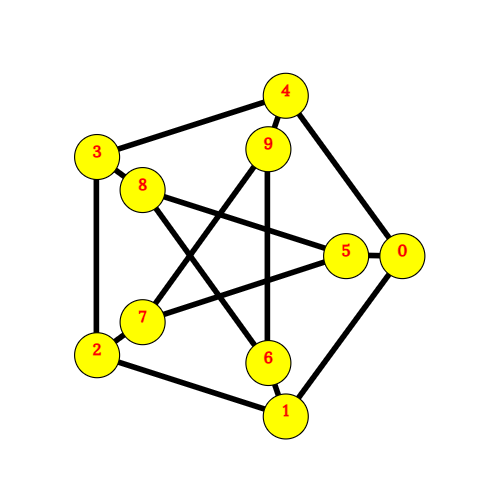
\includegraphics[width=0.5\textwidth]{slike/petersonov.png}
	\caption{Petersonov graf}
	\label{fig:petersonov}
\end{figure}

\begin{figure}[htb]
	\centering
	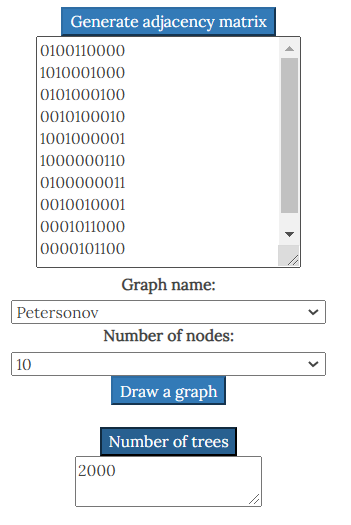
\includegraphics[width=0.5\textwidth]{slike/petersonovbroj.png}
	\caption{Broj razapinjućih stabala Petersonovog grafa}
	\label{fig:petersonov-broj}
\end{figure}

Na slici 6.2 vidi se matrica susjedstva Petersonovog grafa te broj razapinjućih stabala istog. Vidimo da je taj broj 2000.

\subsection{Kotač sa 6 vrhova, \textit{W\textsubscript{5}}}

Na slici 6.3 se vidi graf kotač s 6 vrhova, \textit{W\textsubscript{5}} nacrtan u aplikaciji \textit{Graphelite}.

\begin{figure}[htb]
	\centering
	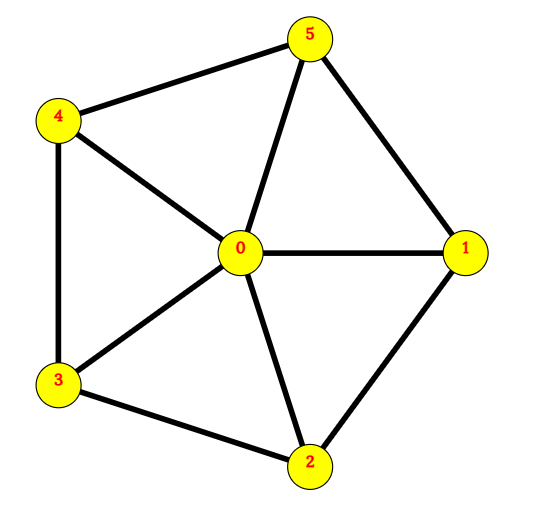
\includegraphics[width=0.5\textwidth]{slike/kotac2.png}
	\caption{Kotač $W_5$}
	\label{fig:kotac}
\end{figure}

\begin{figure}[htb]
	\centering
	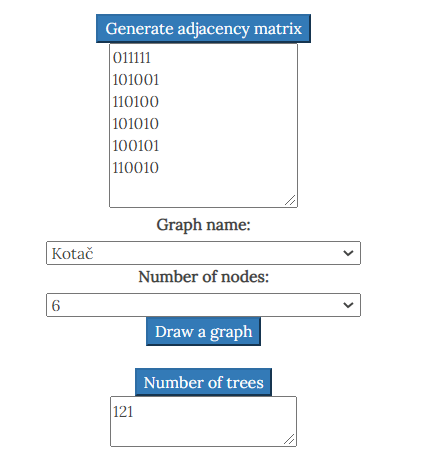
\includegraphics[width=0.5\textwidth]{slike/kotacbroj.png}
	\caption{Broj razapinjućih stabala grafa $W_5$}
	\label{fig:kotac-broj}
\end{figure}

Na slici 6.4 vidi se matrica susjedstva za \textit{W\textsubscript{5}} te broj razapinjućih stabala istog. Vidimo da je taj broj 121.
\chapter{Zaključak}
Zaključak.

\bibliography{literatura}
\bibliographystyle{fer}

\begin{sazetak}
Sažetak na hrvatskom jeziku.

\kljucnerijeci{grafovi, stabla, razapinjuća stabla, matrix-tree teorem}
\end{sazetak}

% TODO: Navedite naslov na engleskom jeziku.
\engtitle{Counting the spanning trees}
\begin{abstract}
Abstract.

\keywords{graphs, trees, spanning trees, matrix-tree theorem}
\end{abstract}

\end{document}
